% MA-SQLGrid original-title reconstruction, Applied Sciences R1.
\documentclass[applsci,article,submit,moreauthors]{Definitions/mdpi}
\firstpage{1}
\makeatletter\setcounter{page}{\@firstpage}\makeatother
\pubvolume{1}\issuenum{1}\articlenumber{0}\pubyear{2026}\copyrightyear{2026}
\datereceived{}\daterevised{}\dateaccepted{}\datepublished{}
\usepackage{booktabs}
\usepackage{algorithm}
\usepackage{algorithmic}
\setlength{\headheight}{20pt}
\setlength{\emergencystretch}{3em}
\newcommand{\masql}{MA-SQLGrid}
\AtBeginDocument{\pdfstringdefDisableCommands{\def\times{x}}}

\Title{MA-SQLGrid: A Robust Multi-Agent Framework for Text-to-SQL in Power Grid Databases}
\Author{Liu Bijing $^{1,2}$, Sun Chenglong $^{1,2}$ and Yang Yong $^{1,2,}$*}
\AuthorNames{Liu Bijing, Sun Chenglong and Yang Yong}
\address{$^{1}$ \quad NARI Group Corporation (State Grid Electric Power Research Institute), Nanjing 211106, Jiangsu Province, China;\\
$^{2}$ \quad Beijing Kedong Electric Power Control System Co., Ltd., Beijing 100080, China}
\corres{Correspondence: Yang Yong; email address to be provided before submission}

\abstract{Natural-language access to power-grid databases requires more than syntactically valid SQL: a query must use the intended schema elements, remain read-only, execute under a defined database state, and expose enough evidence for human review. This paper presents \masql{}, a structured multi-agent framework that separates query analysis, schema grounding, SQL synthesis, safety and execution validation, and counterfactual criticism, with a deterministic adjudicator coordinating the roles through an append-only blackboard. The coordination core rejects unsafe or multi-statement SQL, abstains when no eligible candidate exists, records missing counterfactual evidence as unknown, and seals its trace before any gold query or result is loaded. We integrate this architecture with previously frozen evidence without relabeling earlier single-generation experiments as multi-agent runs. The inherited GridDB study evaluates two quantized local backbones in a paired 2-by-2 prompt design over 180 questions, producing 1440 predictions. No primary factorial execution effect or cross-backbone modifier survived Holm correction, although a composite structural/SQL-operation hint increased projected-column adherence. A separate 700-call component study found a positive presented-value effect for Qwen (+0.1059; 95\% composition-sensitivity interval [0.0282, 0.2013]; adjusted $p=0.0310$) but not Granite; deterministic candidate selection met the declared efficacy rule for neither backbone. On BIRD Mini-Dev, 5000 generation calls yielded 4000 independently re-executed final predictions; the descriptively best methods reached execution accuracy 0.394 for Qwen and 0.236 for Granite. A 15-state GridDB stress test produced logical-AND agreement rates from 0.6212 to 0.8182, with no registered effect surviving correction. Finally, a hash-locked retrospective offline coordination diagnostic found at least two safe candidates with consistent frozen snapshot evidence for 172 of 180 questions. This replay measures candidate-pool coverage only, not accuracy or multi-agent improvement. The evidence supports an auditable framework and a prospectively testable coordination design, not a deployed-system or universal robustness claim.}
\keyword{text-to-SQL; multi-agent systems; power-grid databases; schema grounding; execution validation; counterfactual testing; reproducibility}
\featuredapplication{\masql{} is an experimental read-only decision-support framework for auditable natural-language access to structured power-grid records. Generated SQL and returned source rows require human inspection before consequential use; no operational control, protection, or maintenance decision has been validated.}

\begin{document}

\section{Introduction}

Power-grid organizations maintain relational data about assets, locations, topology, sensor readings, work orders, technicians, and maintenance activity. SQL provides precise access to these records, but it requires knowledge of table names, join keys, identifiers, units, aggregation conventions, and local coding rules. Text-to-SQL systems aim to reduce this access barrier by translating a natural-language request into an executable query. In an engineering workflow, however, a fluent query is not sufficient evidence of correctness. A query can execute while selecting the wrong status field, omitting a required filter, using an unintended join path, or returning the expected number of columns with the wrong content.

Cross-database benchmarks such as Spider and BIRD have made schema generalization and realistic database content central evaluation concerns \cite{yu2018spider,li2023bird}. Schema-aware models, constrained decoding, context selection, decomposition, and execution guidance address different failure surfaces \cite{wang2020ratsql,scholak2021picard,nan2023enhancing,pourreza2023dinsql,talaei2024chess}. These methods also expose a design problem: generation steps are frequently bundled together. A system may change schema serialization, value presentation, domain normalization, structural hints, candidate count, and repair policy simultaneously. An observed score difference then cannot be assigned cleanly to schema linking, reasoning, or validation.

The original \masql{} concept addresses this problem through five specialized roles. A Query Analyst interprets the request, a Schema Cartographer maps it to the database, an SQL Synthesizer packages candidate queries, a Validation Engine checks safety and execution, and a Counterfactual Critic records evidence from named database states. A separate deterministic adjudicator resolves the resulting evidence. This separation makes the trace inspectable: a reviewer can distinguish what the analyst inferred, which schema elements were retained, which candidates were proposed, which candidates executed, and why a final candidate was selected or rejected.

The architecture must nevertheless be separated from the evidence used to evaluate it. The inherited GridDB factorial study was not a multi-agent execution. It used one model generation per question and prompt cell, followed by deterministic parsing, read-only validation, execution, and offline scoring. The BIRD study likewise compared four frozen prompting procedures rather than five interacting agents. These assets can motivate modules, supply baselines, and test replay interfaces, but they cannot be renamed as results of the new coordination core.

This distinction leads to three questions. First, can role-specific handoffs be implemented with a gold-isolated and auditable selection boundary? Second, what do the completed experiments establish about context packages, structural hints, presented values, candidate selection, public-database transfer, and multi-state execution agreement? Third, do the frozen assets contain enough genuinely distinct candidates to support a future matched coordination experiment without new labels or fabricated data? Whether the full multi-agent condition improves execution accuracy under a fixed generation budget remains a prospective question and is not answered by retrospective replay.

The paper makes four contributions. First, it defines a testable five-role coordination core plus a deterministic adjudicator. An append-only blackboard records every typed handoff and emits a canonical SHA-256 digest; gold SQL, gold results, and correctness labels are excluded from all pre-evaluation interfaces. Second, it conservatively integrates a 1440-prediction GridDB factorial experiment, a 700-call component study, a 25,920-row multi-state ledger, and a 5000-call BIRD comparison while retaining their original method identities. Third, it provides a fail-closed retrospective replay that verifies input hashes and audits candidate-pool coverage without reporting accuracy. Fourth, it specifies the safeguards needed for a later budget-matched prospective coordination experiment.

No Spider or WikiSQL experiment is reported, no unsupported large power-grid question--SQL corpus is asserted, and no accuracy advantage is attributed to the new multi-agent core before an independently audited prospective protocol is executed.

\section{Related Work}

\subsection{Text-to-SQL Evaluation and Schema Generalization}

Text-to-SQL systems map a natural-language question and a database schema to a query. Spider established a cross-domain setting with previously unseen databases, drawing attention to table selection, joins, grouping, nesting, and ordering \cite{yu2018spider}. BIRD extends public evaluation toward larger and more content-rich databases \cite{li2023bird}. A benchmark result depends on the exact split, evaluator, database engine, execution boundary, and model configuration. We therefore report only the completed BIRD Mini-Dev protocol and make no claim about public datasets that were discussed but not run.

Exact SQL match and execution evaluation answer different questions. String match can penalize equivalent SQL, whereas result equality can reward nonequivalent queries on an insufficiently discriminating database state. Robust evaluation should retain predicted SQL, record every failure, and specify the state on which equality was observed. \masql{} uses strict result equality for the inherited snapshot experiment and separately reports projected-column conformity and multi-state agreement. Neither auxiliary endpoint is described as semantic certification.

\subsection{Schema Linking, Context Packages, and Output Contracts}

Schema linking connects question spans to tables, columns, values, and foreign-key relations \cite{wang2020ratsql,lei2020reexamining,liu2022semantic}. Full-schema context preserves recall but can increase token cost and distraction. Compact context reduces the search space but risks dropping a required join key or predicate. Value examples can disambiguate coded attributes, while question-derived instructions can identify aggregation, result shape, ordering, or a limit.

The inherited GridDB factorial study isolates two implemented prompt factors: a full-DDL/global-values package versus a compact/domain-grounded package, and absence versus presence of a composite structural/SQL-operation hint. The compact package is not a pure schema-length manipulation because it also changes value presentation and adds corpus-tailored normalization. The hint is not merely formatting because it can include aggregation, grouping, projection, ordering, and limit guidance. We retain these precise labels instead of assigning broader causal interpretations.

Constrained generation and execution guidance reduce invalid candidates. PICARD constrains decoding so inadmissible SQL continuations can be rejected during generation \cite{scholak2021picard}. CHESS combines contextual grounding and SQL synthesis components \cite{talaei2024chess}; other prompt-based methods investigate decomposition and representation choices \cite{nan2023enhancing,sun2023sqlprompt,pourreza2023dinsql}. \masql{} differs at the coordination boundary: its new core accepts externally produced candidates, checks them with deterministic contracts, and records evidence before selection. It does not claim that the current lexical cartographer supersedes learned schema-linking systems.

\subsection{Agentic Decomposition and Auditable Control}

Agentic decomposition can make intermediate decisions explicit, but naming pipeline stages as agents does not establish a multi-agent benefit. Such evidence requires a comparison that holds the model, data, decoding configuration, candidate count, and physical generation budget constant. Otherwise, a multi-candidate system can improve simply because it receives more samples.

\masql{} treats an agent as a role with a typed contract rather than assuming that every role must be a separately hosted model. The Analyst and Cartographer can be deterministic or model-assisted; the Synthesizer can receive candidates from a frozen generator; the Validator uses a fixed read-only policy; the Critic consumes named-state evidence; and the Adjudicator is deterministic. This design allows components to be replaced without changing the blackboard schema and prevents gold-guided selection from being hidden behind an opaque debate label.

\subsection{Power-Grid Data and External Validity}

Power-system datasets combine topology, equipment attributes, measurements, time series, costs, and constraints. RTS-GMLC and SimBench provide reproducible engineering resources that can be transformed into relational structures \cite{barrows2020rts,meinecke2020simbench}. Their availability does not automatically create a text-to-SQL benchmark: intended projections, units, ordering, ties, and reference SQL require semantic review. The current RTS-GMLC, SimBench, and NERC-derived candidates are consequently machine-adjudicated silver resources, not expert gold.

DKA-SQL is a direct power-grid text-to-SQL precedent \cite{bian2025dkasql}. Its published corpus, method, models, and evaluation boundary differ from ours. Because no official implementation was used, the current BIRD protocol is neither a DKA-SQL reproduction nor a head-to-head comparison.

\section{Materials and Methods}

\subsection{Task and Evidence Boundary}

For question $x_i$, read-only database $D_i$, and introspected schema $S_i$, a generator produces one or more candidates
\begin{equation}
\mathcal{Y}_i=\{\widetilde{y}_{i1},\ldots,\widetilde{y}_{ik}\}.
\end{equation}
Each candidate must satisfy a single-statement read-only contract. The accepted leading form is \texttt{SELECT} or \texttt{WITH}; comments, multiple statements, write operations, schema changes, attachments, and pragmas are rejected. A candidate is eligible for adjudication only when it is safe and executable.

The offline evaluator may later compare the selected query with a reference result. Let $E_i=1$ when the selected SQL executes and its result equals the frozen reference result under the registered evaluator, and $E_i=0$ otherwise. Reference SQL, reference results, $E_i$, and any derivative correctness field are forbidden from all five agents and the Adjudicator. Evaluation occurs only after the blackboard is sealed.

\subsection{Data Resources and Provenance}

GridDB-Maintenance-v2 v0.1 is a synthetic SQLite case study with eight tables and 98 rows: \texttt{asset\_types} (6), \texttt{assets} (18), \texttt{grid\_topology} (9), \texttt{locations} (8), \texttt{maintenance\_logs} (8), \texttt{sensor\_readings} (26), \texttt{technicians} (8), and \texttt{work\_orders} (15). It contains 200 natural-language--SQL records: 20 development records and 180 factorial evaluation records. The evaluation records include 66 easy, 91 medium, and 23 hard items and map to 70 normalized gold-SQL structural clusters, of which 58 are singletons. The evaluation partition had been visible during project development; it is a controlled finite-set case study, not a sealed production benchmark.

BIRD Mini-Dev contributes 500 public items over 11 SQLite databases. The authorized protocol froze item and method order, prompts, two local model files, evaluator behavior, Python 3.10.11/SQLite 3.40.1, and zero retries. Each backbone made 2500 calls and produced 2000 final predictions. An independent audit re-executed all 4000 predictions and 500 gold queries with zero score mismatches. Two earlier failed attempts, totaling 2476 physical calls, remain immutable incidents and are excluded from scores.

The GridDB reliability release contains 18 states: the canonical snapshot, three insertion permutations, and 14 additional schema-valid stress states. The scorer produced 25,920 prediction-state rows ($1440\times18$). A prediction-blinded automated protocol admitted a 66-question subset for the primary 15-state analysis and retained 114 order-sensitive questions as diagnostics. These constructed states are not operator-certified grid snapshots.

Artifacts are labeled Inherited, Recomputed, New, or Diagnostic. The coordination core is implementation evidence and its replay is Diagnostic. Neither is a New execution-accuracy result.

\subsection{Five-Agent Coordination Framework}

\masql{} comprises five specialist roles coordinated by a deterministic controller. Figure~\ref{fig:coordination} is derived from the implemented source rather than an aspirational free-form agent diagram. The controller is not a sixth reasoning model: it orders calls, applies the registered rule, and seals the trace. Messages receive consecutive sequence numbers, and the complete trace is serialized canonically to a SHA-256 digest.

\begin{figure}[htbp]
\centering
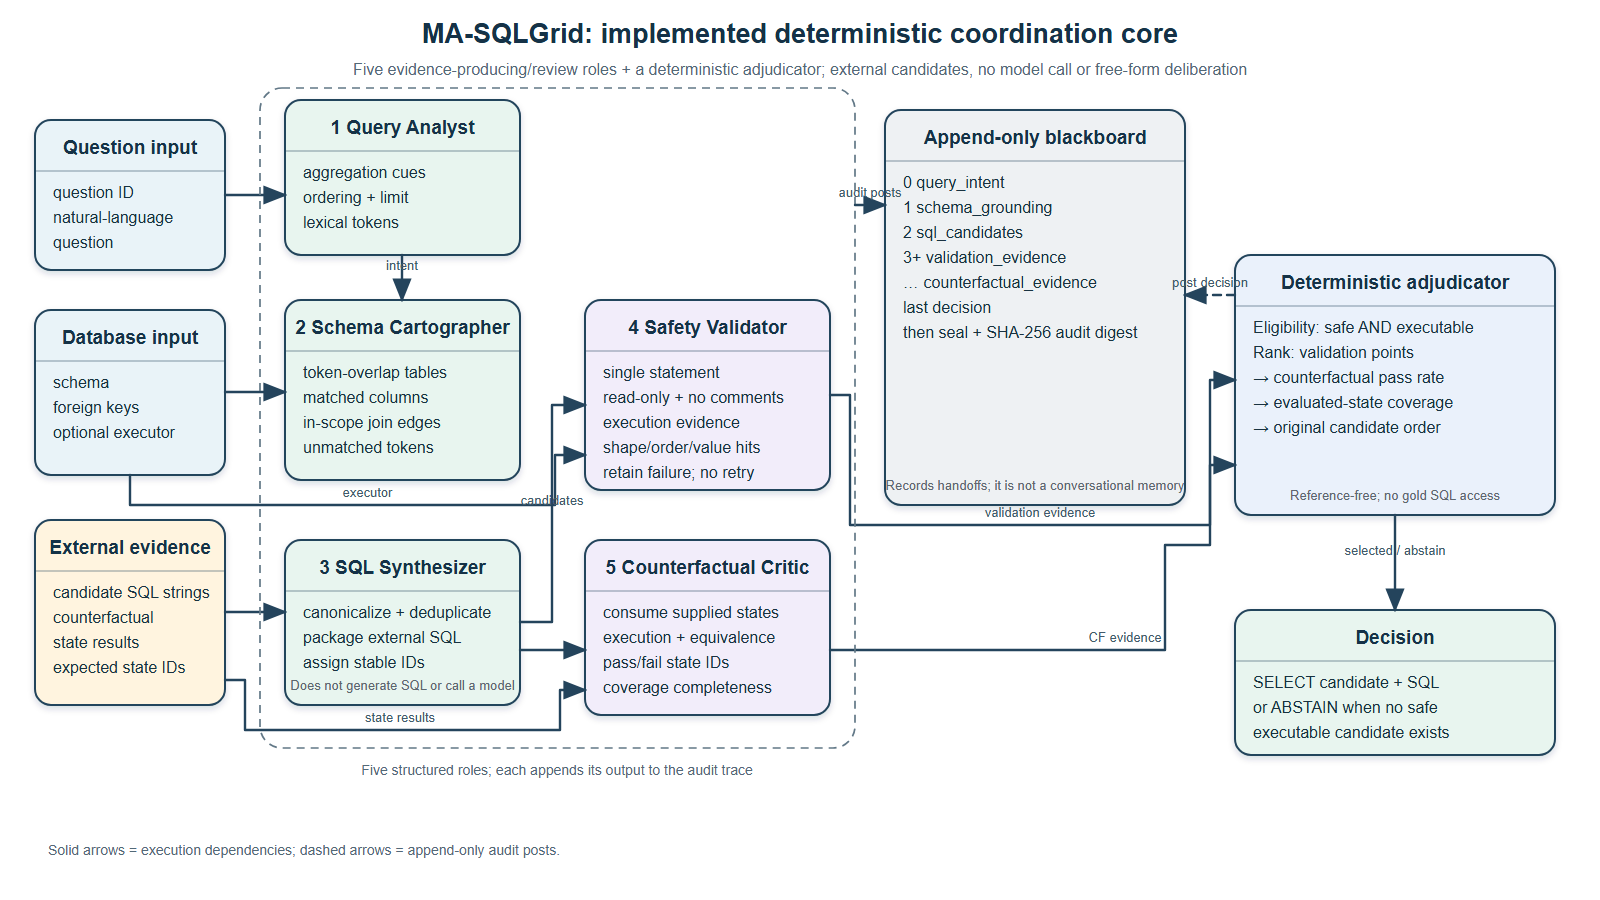
\includegraphics[width=0.98\textwidth]{figures/fig_ma_sqlgrid_implemented_coordination_r1_qa3.png}
\caption{Implemented \masql{} coordination core. Five evidence-producing or review roles communicate through an append-only blackboard. SQL candidates and state evidence are supplied externally; the deterministic Adjudicator selects a safe executable candidate or abstains. Gold SQL is outside the sealed coordination boundary.}
\label{fig:coordination}
\end{figure}

The \textbf{Query Analyst} produces a structured question-only intent record containing lexical tokens, detected aggregations, ordering requirements, and an explicit limit when present. It does not select SQL or see correctness. The \textbf{Schema Cartographer} maps lexical intent to tables, columns, and foreign-key edges. The current skeleton uses deterministic overlap and records unmatched tokens; a richer GridDB adapter adds disclosed domain rules and graph expansion.

The \textbf{SQL Synthesizer} packages externally produced SQL strings. It contains no model client, performs no hidden API call, canonicalizes whitespace and semicolons, removes exact duplicates without changing first occurrence, and assigns stable identifiers. The \textbf{Validation Engine} applies the read-only policy and records safety, executability, output-shape, ordering, presented-value hits, errors, and an optional result hash. Missing execution evidence makes a candidate ineligible rather than valid by assumption.

The \textbf{Counterfactual Critic} consumes named state results, rejects duplicate state identifiers, and records evaluated, passed, and failed states. Missing states remain unknown. Existing formal-v5 labels compare predictions with gold; using them during selection would leak evaluator information. The replay therefore passes no such labels to the Critic and records zero reference-free counterfactual coverage.

\subsection{Deterministic Adjudication and Abstention}

Eligibility requires safety and successful execution. The implemented rule assigns 40 validation points for safety, 40 for execution, 10 for shape conformity, 5 for ordering conformity, and up to 5 for presented-value hits. Ties are resolved by counterfactual pass rate when available, then evaluated-state coverage, then original candidate order. If no candidate is eligible, the controller abstains. In the retrospective diagnostic, adjudication is attempted only when at least two distinct candidates are safe and supported by consistent frozen T0 evidence.

\begin{algorithm}[htbp]
\caption{Gold-isolated deterministic coordination}
\label{alg:coordination}
\begin{algorithmic}[1]
\REQUIRE question $x_i$, schema $S_i$, external candidates $\mathcal{Y}_i$, read-only executor, named state evidence
\STATE post structured intent and schema grounding to the append-only blackboard
\STATE canonicalize and deduplicate externally produced candidates
\FOR{each candidate $y\in\mathcal{Y}_i$}
  \STATE apply single-statement read-only validation
  \STATE record execution and available reference-free state evidence
\ENDFOR
\IF{no safe executable candidate exists}
  \STATE abstain
\ELSE
  \STATE apply the fixed validation, state-evidence, coverage, and order rule
\ENDIF
\STATE post the decision and seal the blackboard
\STATE load reference results only for offline evaluation
\end{algorithmic}
\end{algorithm}

\subsection{Inherited GridDB Factorial Design}

The paired design crosses context package $c\in\{0,1\}$ and composite hint $h\in\{0,1\}$. F00 uses full DDL and global values without the hint; F01 adds the hint; F10 uses compact domain-grounded context without the hint; and F11 combines compact context and the hint. The same 180 questions appear in all four cells for each backbone, yielding 720 Qwen and 720 Granite predictions.

Qwen2.5-Coder-7B Q4\_K\_M and Granite-3.3-8B Q4\_K\_M were run at temperature zero with fixed snapshots. Each prompt produced exactly one response. The parser retained the first SQL candidate through the first semicolon; the validator then applied the read-only policy. There was no candidate ranking, multi-agent negotiation, or repair in this experiment.

Strict execution equality is primary. A common-target projected-column indicator is a secondary manipulation check. Paired finite-set contrasts use normalized-SQL clusters as dependence proxies, registered sign-flip tests, composition-sensitivity bootstrap intervals, and Holm correction. The intervals describe sensitivity to the observed corpus composition, not population confidence.

\subsection{Component, Multi-State, and Public Protocols}

The separately frozen component study contains 700 scored calls. E1 compares candidate generation with and without presented value evidence. E2 requests up to three candidates and compares a deterministic reference-answer-independent selector with the first candidate. Selection is sealed before gold loading. Rescue, harm, and oracle-at-three are descriptive; oracle-at-three is a gold-only upper-bound diagnostic.

The v5 reliability protocol reproduced all 1440 T0 labels and then executed every prediction over 18 states. The primary 66-question analysis uses a logical-AND endpoint over 15 semantic states. A prediction passes only when it agrees with the reference on every included state. The nine registered contrasts form a separate Holm family; with only 12 structural clusters, all $2^{12}=4096$ sign assignments are enumerated.

The BIRD protocol compares direct prompting, decomposition, schema selection, and bounded execution repair. Each method has a fixed call pattern and zero retries. Pairwise differences use exact database-cluster sign randomization across 11 databases and Holm correction.

\subsection{Retrospective Offline Coordination Diagnostic}

The replay verifies SHA-256 for two 720-row prediction ledgers and the 25,920-row formal-v5 ledger before reading them. For each question it pools the eight existing outputs from two backbones and four prompt cells, canonicalizes SQL, and removes duplicates. Frozen T0 fields provide execution and metadata-shape evidence. The Critic records counterfactual evidence as unavailable because existing state-agreement labels are gold-relative.

This is a coverage diagnostic. Candidates were generated under different models and prompt packages; the pool is not a deployable, matched multi-agent run. No selected output is compared with gold to produce an accuracy number.

\section{Results}

\subsection{Complete GridDB Cell Results}

All 1440 scheduled predictions are present, and independent SQLite re-execution reproduced the stored execution verdicts. Table~\ref{tab:cells} reports strict execution equality.

\begin{table}[htbp]
\caption{Strict execution equality over 180 GridDB questions per cell.}
\label{tab:cells}
\centering
\small
\setlength{\tabcolsep}{4pt}
\begin{tabular}{lcccc}
\toprule
Backbone & F00 full/no hint & F01 full/hint & F10 compact/no hint & F11 compact/hint\\
\midrule
Qwen & 0.4222 & 0.7167 & 0.4333 & 0.6000\\
Granite & 0.4278 & 0.5556 & 0.4111 & 0.6000\\
\bottomrule
\end{tabular}
\end{table}

\begin{figure}[htbp]
\centering

\includegraphics[width=0.94\textwidth]{figures/results/fig01_v2_cells.pdf}
\caption{Audited GridDB cell point estimates. Each cell contains all 180 attempts; the figure is descriptive and does not replace registered factorial contrasts.}
\label{fig:cells}
\end{figure}

The common-target projected-column diagnostic is 0.5222 in F00 for both backbones. Qwen obtains 0.9667, 0.5889, and 0.9611 in F01, F10, and F11; Granite obtains 0.8778, 0.5667, and 0.9222. Returning the requested number of columns is therefore easier than returning the intended rows. In Qwen F01, projected-column conformity is 0.9667 while execution equality is 0.7167.

\subsection{Factorial Effects and Multiplicity}

For Qwen, the composite-hint execution effect is +0.2306, the package--hint interaction is $-0.1278$, and the compact-package main effect is $-0.0528$. Granite's corresponding estimates are +0.1583, +0.0611, and +0.0139. Zero of nine primary execution tests survives Holm correction. Qwen's hint effect has raw/adjusted $p=0.01372/0.09604$, its interaction $0.00919/0.07352$, and the cross-backbone hint modifier $0.00640/0.05760$. No primary factorial execution effect or modifier is therefore described as statistically nonzero.

In the separately corrected secondary family, the common-target hint effects survive: +0.4083 for Qwen (adjusted $p=0.000090$) and +0.3556 for Granite (adjusted $p=0.01944$). Because the hint supplies structural information later scored by this endpoint, these are manipulation-check results, not independent semantic evidence.

\subsection{Component Results}

The component run completed all 700 scored calls. Presented value evidence increased Qwen first-candidate execution equality by +0.1059 over 170 eligible questions (95\% composition-sensitivity interval [+0.0282, +0.2013], adjusted $p=0.0310$). Granite's estimate was zero with an interval spanning zero. The cross-backbone modifier did not meet the registered rule, so the Qwen result is not replicated across backbones.

The deterministic selector changed 24 Qwen and 36 Granite choices. Relative to the first candidate, it rescued eight and harmed one Qwen question, and rescued ten while harming none for Granite. Execution effects were +0.0389 and +0.0556; neither survived its two-test Holm family. Oracle-at-three values of 0.6389 and 0.4667 are gold-only diagnostics and are not deployable selector results.

\begin{figure}[htbp]
\centering

\includegraphics[width=0.92\textwidth]{figures/results/figure_01_primary_effects.pdf}
\caption{Prospectively frozen component effects. Intervals describe composition sensitivity; the registered decision also requires multiplicity-adjusted evidence.}
\label{fig:components}
\end{figure}

\subsection{Multi-State Reliability Results}

The v5 scorer produced all 25,920 registered rows, and its T0 slice reproduced 1440/1440 snapshot labels. Across the 66-question automatic subset, 15-state logical-AND rates range from 0.6212 (Granite F01) to 0.8182 (Granite F00). All nine Holm-adjusted values equal 1.0000 under exact cluster-sign enumeration. No context, hint, interaction, or cross-backbone multi-state effect meets the declared rule. These rates characterize agreement over constructed witness states, not population accuracy or human-certified equivalence.

\begin{figure}[htbp]
\centering
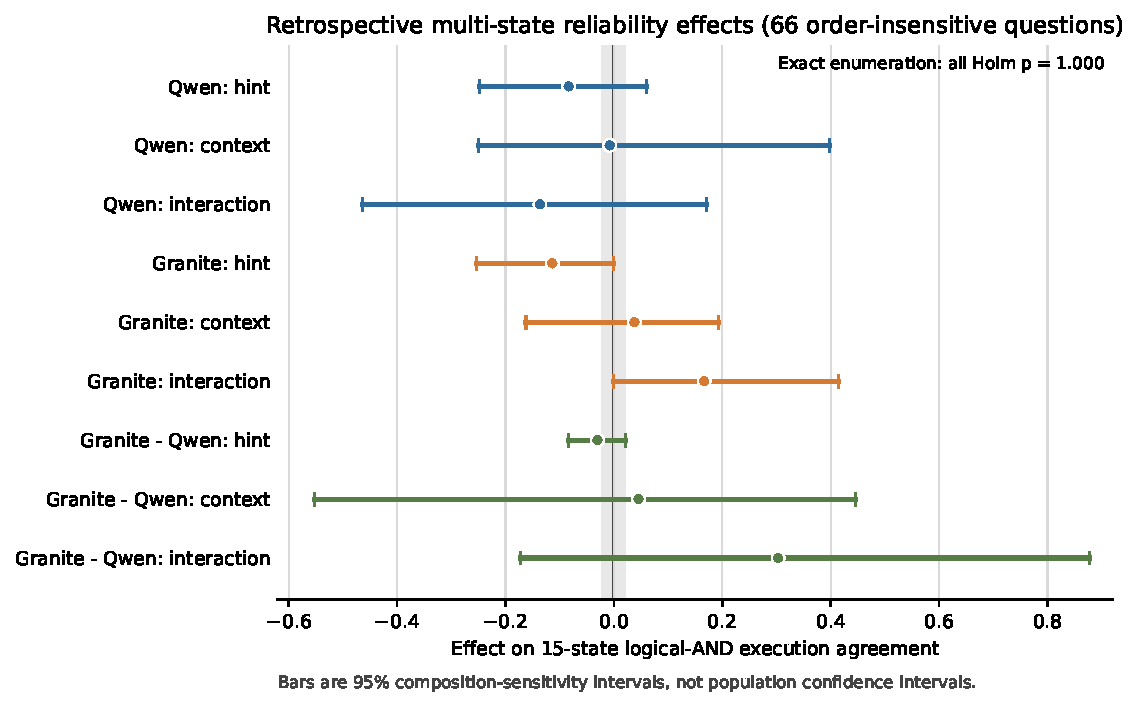
\includegraphics[width=0.92\textwidth]{figures/results/fig04_semantic_reliability.pdf}
\caption{GridDB multi-state logical-AND agreement for the prediction-blinded automatic subset. The endpoint is a constructed-state robustness diagnostic.}
\label{fig:multistate}
\end{figure}

\subsection{Public BIRD Results}

Across 500 BIRD Mini-Dev items, Qwen schema selection is descriptively best at 0.394 execution accuracy, followed by direct prompting at 0.378, bounded execution repair at 0.348, and decomposition at 0.302. Granite bounded execution repair is descriptively best at 0.236; its other methods range from 0.202 to 0.210. After Holm adjustment, Qwen decomposition is 0.076 below direct prompting (adjusted $p=0.0430$), and schema selection is 0.092 above decomposition (adjusted $p=0.0117$). No Granite contrast survives correction. Different method orders across the two snapshots argue against a universal prompting recipe.

\subsection{Retrospective Replay Coverage}

The replay audited all 180 GridDB questions without a generation call. At least two distinct frozen SQL candidates were present for 173 questions. After safety checks and binding to consistent T0 execution evidence, 172 questions had at least two eligible candidates and entered retrospective adjudication. Seven failed closed because only one unique SQL remained, and one failed because fewer than two candidates were eligible.

\begin{table}[htbp]
\caption{Retrospective offline coordination diagnostic coverage. Counts are not accuracy and do not estimate multi-agent improvement.}
\label{tab:replay}
\centering
\begin{tabular}{lr}
\toprule
Coverage gate & Questions\\
\midrule
Audited & 180\\
At least two unique frozen SQL candidates & 173\\
At least two eligible candidates & 172\\
Retrospectively adjudicated & 172\\
Failed closed: one unique candidate & 7\\
Failed closed: fewer than two eligible candidates & 1\\
Reference-free counterfactual evidence available & 0\\
\bottomrule
\end{tabular}
\end{table}

Unique candidate counts ranged from one to eight: 1 (7 questions), 2 (19), 3 (15), 4 (18), 5 (27), 6 (23), 7 (45), and 8 (26). These counts show that frozen assets can populate the coordination interfaces for most questions. They do not show that retrospectively selected SQL is correct. No retrospective accuracy, execution gain, rescue rate, or multi-agent superiority is reported.

\section{Discussion}

\subsection{What the Evidence Supports}

The combined evidence supports three bounded findings. First, explicit structural and SQL-operation instructions strongly alter projected-column adherence, but surface conformity does not establish correct execution. Second, presented value evidence can matter for one frozen model snapshot while showing no effect for another. Third, candidate selection and prompting are backbone-dependent: the component selector did not meet its registered efficacy rule, and the descriptively best BIRD method differed between Qwen and Granite.

These findings justify separating intent, schema grounding, synthesis, validation, and robustness evidence. They do not establish that five roles are superior to one call. The architecture's current value is methodological: typed contracts, explicit eligibility, deterministic selection, abstention, incident retention, and a sealed gold boundary make a future comparison reproducible and falsifiable.

\subsection{Interpreting the Retrospective Replay}

The replay asks whether inherited ledgers contain enough distinct executable candidates to exercise the coordination interfaces. For 172 of 180 questions, they do. This reduces implementation risk and identifies eight fail-closed cases that require a registered fallback or a new matched generation policy.

The replay cannot estimate a coordination effect. Its pool mixes two backbones and four prompt packages, so generation condition and diversity are confounded. It also lacks reference-free counterfactual equivalence evidence. Post hoc gold scoring of selected outputs would remain exploratory and cannot substitute for a prospective matched comparison.

\subsection{Power-Grid Use and Reproducibility}

Read-only execution, syntactic validity, and result-shape conformity are necessary safeguards, not operational certification. A safe query can still return the wrong assets, omit time bounds, misinterpret codes, or mishandle ties. Multi-state witnesses reduce accidental snapshot equality but cannot cover all distributions or schema changes. Generated SQL and returned source rows require human inspection before any maintenance, protection, dispatch, or asset-management decision.

Negative results are part of the contribution. Zero of nine primary factorial execution tests survives correction. The deterministic component selector meets its efficacy rule for neither snapshot. No registered multi-state effect survives correction. Granite and Qwen do not share the same best BIRD method. Immutable ledgers, direct re-execution, registered test families, portable manifests, and explicit incidents preserve these outcomes rather than collapsing them into a success narrative.

\section{Limitations and Future Work}

The primary domain corpus is one synthetic database with eight tables, 98 rows, and 180 evaluation questions. Its evaluation partition was visible during development. The 70 structural groups are dependence proxies, and 58 are singletons. Results cannot be generalized to production schemas, permissions, missing-data patterns, units, access-control policies, or workloads.

Only two quantized local snapshots were evaluated. Model family, size, quantization, serving software, and serialization may interact. The compact package bundles schema reduction, values, normalization, and serialization; the hint bundles projection, aggregation, grouping, ordering, and limit rules. The inherited factorial experiment identifies package effects rather than contributions of individual internal rules.

The five-role core is implemented and unit-tested but has not completed a prospectively frozen generation experiment. Its Analyst and Cartographer are deterministic skeletons, its Synthesizer packages external candidates, and its adjudication weights have not been independently optimized. The retrospective replay is not an accuracy experiment. Existing formal-v5 agreement labels are gold-relative and intentionally excluded from selection.

RTS-GMLC, SimBench, and NERC question--SQL assets remain machine-adjudicated silver data. Qualified review is required for intended projections, units, ordering, tie handling, and result granularity before external accuracy is reported.

Future work should execute a new hash-locked, budget-matched comparison of four conditions: a single direct candidate; staged question/schema handoffs with one candidate; a fixed multi-candidate budget with validation and adjudication but no counterfactual evidence; and the same candidate pool with a pre-registered reference-free state or invariant suite. Model snapshot, question order, database state, decoding, candidate count, and physical calls must be held constant for the primary contrast. The protocol must pre-register execution accuracy, valid SQL, abstention, token and latency endpoints, clustered inference, multiplicity, and incident retention. Until that experiment is authorized and completed, the manuscript makes no multi-agent performance claim.

Further work can replace lexical grounding with a trained schema linker, add a low-confidence full-schema fallback, compare deterministic adjudication with budget-matched voting, and evaluate abstention calibration. Every change should receive a new protocol identity rather than modifying a completed run.

\section{Conclusions}

\masql{} reframes power-grid text-to-SQL as an auditable coordination problem. Five specialist roles separate question analysis, schema mapping, candidate packaging, safety and execution validation, and counterfactual criticism. A deterministic controller records their handoffs, selects only eligible candidates, and abstains when evidence is insufficient. This restores the intent of the original title while maintaining a strict boundary between implementation and demonstrated performance.

The inherited experiments provide a substantial but bounded evidence base. The 1440-prediction GridDB study shows strong projected-column instruction uptake but no primary execution effect surviving Holm correction. The 700-call component study supports presented values for one Qwen snapshot, not Granite, and does not validate the selector under its registered rule. The 25,920-row state study finds no corrected factorial reliability effect. The 5000-call BIRD protocol supplies a public comparison whose best method depends on the backbone. The retrospective replay confirms candidate coverage for 172 of 180 questions while deliberately reporting no accuracy or counterfactual gain.

The next scientific gate is prospective: freeze a budget-matched coordination comparison, seal blackboards before gold evaluation, retain every failure, and report the result whether positive or negative. Until that gate is completed, \masql{} is a reproducible framework with inherited component evidence and a tested coordination interface, not a proven superiority result or deployed power-grid system.

\supplementary{The reproducibility package contains hash-bound prompts, predictions, scores, frozen protocols, incident records, independent re-execution audits, statistical tables, figure sources, the multi-state release, BIRD v1.1 ledgers, the five-role coordination core, unit tests, and the retrospective diagnostic ledger and manifest. Public code and license-cleared materials are available at \url{https://github.com/gaoxingkele/ma-sqlgrid}; restricted materials are available under the Data Availability Statement.}
\authorcontributions{Conceptualization, B.L. and Y.Y.; methodology, B.L.; software, B.L.; validation, B.L. and C.S.; formal analysis, B.L. and C.S.; investigation, B.L. and C.S.; resources, Y.Y.; data curation, B.L. and C.S.; writing---original draft preparation, B.L.; writing---review and editing, C.S. and Y.Y.; visualization, B.L.; supervision, Y.Y.; project administration, Y.Y.; funding acquisition, Y.Y. All authors have read and agreed to the published version of the manuscript.}
\funding{This research was funded by the Science and Technology Project of NARI Group Corporation (State Grid Electric Power Research Institute), grant number 521300250006.}
\institutionalreview{Not applicable. This study did not involve human participants or animals.}
\informedconsent{Not applicable.}
\dataavailability{Public project code and license-cleared reproducibility materials are available at \url{https://github.com/gaoxingkele/ma-sqlgrid}. BIRD Mini-Dev remains available from its public provider. Owing to third-party licensing restrictions, materials not included in the public repository, including restricted source records and source-dependent RTS-GMLC and SimBench artifacts, are available from the corresponding author upon reasonable request for editorial and peer-review verification, subject to third-party permission and applicable licenses. The submission-version verification package includes hash-bound prompts, predictions, scores, audits, generated tables and figures, BIRD Mini-Dev v1.1 ledgers, the post-run audit, and machine-adjudicated external-review artifacts.}
\acknowledgments{During preparation of this manuscript, the authors used OpenAI Codex (GPT-5-based) for drafting, editing, code review, and reproducibility checks. The authors reviewed and edited the outputs and take full responsibility for the publication. Machine-generated external question--SQL candidates were not treated as human or domain-expert ground truth in the quantitative evaluation.}
\conflictsofinterest{The authors declare no conflicts of interest. The funder had no role in the design of the study; in the collection, analysis, or interpretation of data; in the writing of the manuscript; or in the decision to publish the results.}

\begin{adjustwidth}{-\extralength}{0cm}
\reftitle{References}
\bibliography{references_verified}
\PublishersNote{}
\end{adjustwidth}
\end{document}
